\documentclass[12pt, titlepage]{article}
\usepackage{graphicx}
\usepackage{amsmath}
\usepackage{esint}
\usepackage{tcolorbox}
\usepackage{parskip}
\usepackage[]{fancyhdr}
\usepackage{pgfplots}
\usepackage{mdframed}
\usepackage{multicol}
\pgfplotsset{compat=1.18}
\setlength{\headheight}{15pt}
\tcbuselibrary{breakable}

\title{Magnetic Fields and Electromagnetism}
\author{Matthew Pan}
\date{April 2025}

\newtcolorbox{Problem}{colback=blue!5!white,colframe=blue!50!black,title=Problem, breakable=true}

\begin{document}

\pagestyle{fancy}

\fancyhead{}
\fancyhead[L]{Pan}
\fancyhead[R]{\thepage}

\maketitle

\section*{12.1 magnetic Fields}

A magnetic field is a vector field that describes the magnetic force exerted on moving charges, electric currents, or magnetic materials. On a microscopic level, magnetic dipoles are created by the circular or rotational motion of electric charges, such as electrons. Since magnetic fields are created by magnetic dipoles, which always have a north and a south pole, magnetic field lines always form a closed loop: north to south outside a magnet and south to north inside a magnet. Magnetic fields can never occur as a monopole, meaning the north and south poles of a magnet cannot be separated.

Because magnetic poles always occur as dipoles, the net magnetic field through any closed surface will always be zero. This is Maxwell's second equation.
\begin{equation*}
    \oiint B \cdot dA = 0
\end{equation*}

Magnetic permeability describes a substance's ability to form internal magnetic fields, represented by $\mu$. A material's relative permeability is its actual permeability divided by the permeability of free space.
\begin{equation*}
    \mu_r = \frac{\mu}{\mu_0}
\end{equation*}

The E\&M course teaches three types of magnetism:
\begin{enumerate}
    \item \textbf{Ferromagnetism} - Found in permanent magnets - the magnetic moments continue to be aligned after exposure to a magnetic field, producing its own field. 
    \item \textbf{Paramagnetism} - A weak alignment of magnetic moments within a material when exposed to an external magnetic field. the moments become disaligned when the field is removed. $\mu_r$ is close to 1.
    \item \textbf{Diamagnetism} - A weak alignment of magnetic moments within a material when exposed to an external magnetic field. The magnetic moments align in the opposite direction as the external field. The moments become disaligned when the field is removed. This property is present in all materials, but is usually neglible unless no other magnetic effects are present. $\mu_r$ is close to 1.
\end{enumerate}

\section*{12.2 Magnetism and Moving Charges}

Moving charge carriers produce magnetic fields. The magnitude and direction of a magnetic field is defined by the Biot-Savart Law:
\begin{equation*}
    d\vec{B} = \frac{\mu_0}{4\pi}\frac{Id\vec{l}\times\hat{r}}{r^2}
\end{equation*}

In this section, we are most concerned about finding the direction of the magnetic field. We will find the magnitude in later sections.

Notice the cross product in the Biot-Savart law---we can find this using the right hand rule. When finding the cross product $\vec{C}=\vec{A}\times\vec{B}$, your pointer finger represents $\vec{A}$, your middle finger represents $\vec{B}$, and your thumb represents $\vec{C}$. Always keep your thumb orthogonal to your pointer and middle fingers.

We can apply a simplified version of the Biot-Savart law to find the \textbf{direction of a magnetic field only}.
\begin{equation*}
    B=v\times\hat{r}
\end{equation*}
Where
\begin{itemize}
    \item \textbf{$B$} is the direction of the magnetic field
    \item \textbf{$v$} is the direction that the charged particle is traveling in 
    \item \textbf{$\hat{r}$} points away from moving charge towards where you are measuring the magnetic field
\end{itemize}

\begin{center}
    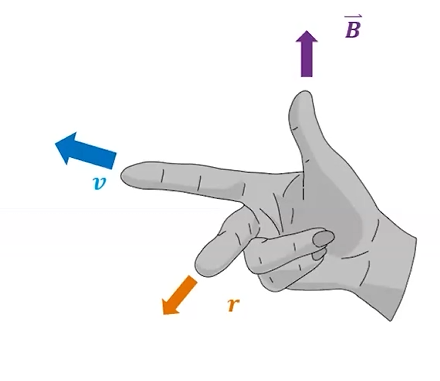
\includegraphics[width=6cm]{media/rh1.png}
\end{center}

When we apply this to many points around the moving charge, we find that the magnetic field forms a concentric circles around the charge, leading us to the next right hand rule.

When making a ``thumbs up'' hand gesture, the thumb points in the direction of the current, the the other fingers curl in the direction that the field circles in around the moving charged object.
\begin{center}
    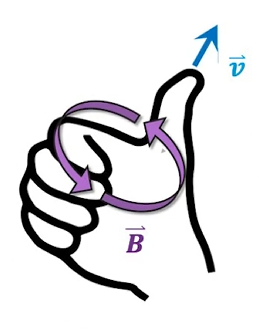
\includegraphics[width=4cm]{media/rh2_2.png}
    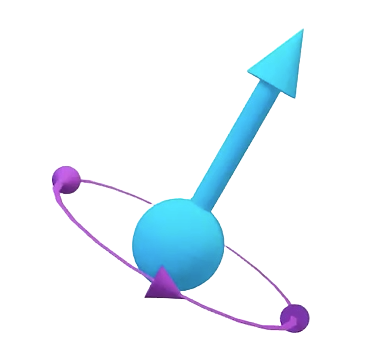
\includegraphics[width=4cm]{media/rh2.png}
\end{center}
\end{document}